%
% linear.tex
%
% (c) 2021 Prof Dr Andreas Müller, OST Ostschweizer Fachhochschule
%
\section{Lineare Algebra
\label{buch:grundlagen:section:linearealgebra}}
\rhead{Lineare Algebra}
In diesem Abschnitt tragen wir die bekannten Resultate der linearen
Algebra zusammen.
Meistens lernt man diese zuerst für Vektoren und Gleichungssyteme mit
reellen Variablen.
In der linearen Algebra werden aber nur die arithmetischen
Grundoperationen verwendet, es gibt also keinen Grund, warum sich
die Theorie nicht über einem beliebigen Zahlenkörper entwickeln
lassen sollte.
Die in Kapitel~\ref{buch:chapter:endliche-koerper} untersuchten
endlichen Körper sind zum Beispiel besser geeignet für Anwendungen in
der Kryptographie oder für die diskrete schnelle Fourier-Transformation.
Daher geht es in diesem Abschnitt weniger darum alles herzuleiten,
sondern vor allem darum, die Konzepte in Erinnerung zu rufen und
so zu formulieren, dass offensichtlich wird, dass alles mit einem
beliebigen Zahlkörper $\Bbbk$ funktioniert.

%
% Vektoren
%
\subsection{Vektoren
\label{buch:grundlagen:subsection:vektoren}}
Koordinatensysteme haben ermöglicht, Punkte als Zahlenpaare zu beschreiben.
Dies ermöglicht, geometrische Eigenschaften als Gleichungen auszudrücken,
aber mit Punkten kann man trotzdem noch nicht rechnen.
Ein Vektor fasst die Koordinaten eines Punktes in einem Objekt zusammen,
mit dem man auch rechnen und zum Beispiel Parallelverschiebungen
algebraisieren kann.
Um auch Streckungen ausdrücken zu können, wird auch eine Menge von 
Streckungsfaktoren benötigt, mit denen alle Komponenten eines Vektors
multipliziert werden können.
Sie heissen auch {\em Skalare} und liegen in $\Bbbk$.

\subsubsection{Zeilen- und Spaltenvektoren}
Vektoren sind Tupel von Elementen aus $\Bbbk$.

\begin{definition}
Ein $n$-dimensionaler {\em Spaltenvektor} ist ein $n$-Tupel von Zahlen aus
$\Bbbk$ geschrieben als
\[
v = \begin{pmatrix} v_1\\v_2\\\vdots\\v_n\end{pmatrix}
\in \Bbbk^n.
\]
Ein $m$-dimensionaler {\em Zeilenvektor} wird geschrieben als
\[
u = \begin{pmatrix}u_1&u_2&\dots&u_m\end{pmatrix} \in \Bbbk^m.
\]
\end{definition}

Für Vektoren gleicher Dimension sind zwei Rechenoperationen definiert.
Die {\em Addition von Vektoren} $a,a\in\Bbbk^n$  und die Multiplikation
eines Vektors mit einem Skalar $\lambda\in\Bbbk$ erfolgt elementweise:
\[
a+b
=
\begin{pmatrix}a_1\\\vdots\\a_n\end{pmatrix}
+
\begin{pmatrix}b_1\\\vdots\\b_n\end{pmatrix}
=
\begin{pmatrix}a_1+b_1\\\vdots\\a_n+b_n\end{pmatrix},
\qquad
\lambda a
=
\lambda
\begin{pmatrix}a_1\\\vdots\\a_n\end{pmatrix}
=
\begin{pmatrix}\lambda a_1\\\vdots\\\lambda a_n\end{pmatrix}.
\]
Die üblichen Rechenregeln sind erfüllt, nämlich 
\begin{equation}
\begin{aligned}
&\text{Kommutativität:}
&
a+b&=b+a
&&
&&\forall a,b\in V
\\
&\text{Assoziativgesetze:}
&
(a+b)+c&=a+(b+c)
&
(\lambda\mu)a&=\lambda(\mu a)
&&\forall a,b,c\in V,\; \lambda,\mu\in\Bbbk
\\
&\text{Distributivgesetze:}
&
\lambda(a+b)&=\lambda a + \lambda b
&
(\lambda+\mu)a&=\lambda a + \mu a
&&\forall a,b\in V,\; \lambda,\mu\in\Bbbk.
\\
\end{aligned}
\label{buch:vektoren-und-matrizen:eqn:vrgesetze}
\end{equation}
Diese Gesetze drücken aus, dass man mit Vektoren so rechnen kann, wie man
das in der Algebra gelernt hat, mit der einzigen Einschränkung, dass
man Skalare immer links von Vektoren schreiben muss.
Die Distributivgesetze zum Beispiel sagen, dass man Ausmultipilizieren
oder Ausklammern kann genauso wie in Ausdrücken, die nur Zahlen enthalten.

Man beachte, dass es im allgemeinen kein Produkt von Vektoren gibt.
Das aus der Vektorgeometrie bekannte Vektorprodukt ist eine Spezialität
des dreidimensionalen Raumes, es gibt keine Entsprechung dafür in anderen
Dimensionen.

\subsubsection{Standardbasisvektoren}
In $\Bbbk^n$ findet man eine Menge von speziellen Vektoren, durch die
man alle anderen Vektoren ausdrücken kann.
Mit den sogenannten {\em Standardbasisvektoren}
\[
e_1=\begin{pmatrix}1\\0\\\vdots\\0\end{pmatrix},
e_2=\begin{pmatrix}0\\1\\\vdots\\0\end{pmatrix},
\dots,
e_n=\begin{pmatrix}0\\0\\\vdots\\1\end{pmatrix}
\]
kann der Vektor $a\in\Bbbk^n$ als
\[
a
=
\begin{pmatrix}a_1\\a_2\\\vdots\\a_n\end{pmatrix}
=
a_1 \begin{pmatrix}1\\0\\\vdots\\0\end{pmatrix}
+
a_2 \begin{pmatrix}0\\1\\\vdots\\0\end{pmatrix}
+
\dots
+
a_n \begin{pmatrix}0\\0\\\vdots\\1\end{pmatrix}
=
a_1e_1+a_2e_2+\dots+a_ne_n
\]
ausgedrückt werden.

\subsubsection{Vektorraum}
Die Rechnungen, die man gemäss der Rechengesetze
\eqref{buch:vektoren-und-matrizen:eqn:vrgesetze}
anstellen kann, verlangen nicht, dass Elemente $a$ und $b$, mit denen man
da rechnet, Zeilen- oder Spaltenvektoren sind.
Jede Art von mathematischem Objekt, mit dem man so rechen kann,
kann als (abstrakter) Vektor betrachtet werden.

\begin{definition}
Eine Menge $V$ von Objekten, auf der zwei Operationen definiert,
nämlich die Addition, geschrieben $a+b$ für $a,b\in V$ und die
Multiplikation mit Skalaren, geschrieben $\lambda a$ für $a\in V$ und 
$\lambda\in \Bbbk$, heisst ein {\em $\Bbbk$-Vektorraum} oder {\em Vektorraum
über $\Bbbk$} (oder
einfach nur {\em Vektorraum}, wenn $\Bbbk$ aus dem Kontext klar sind),
wenn die Rechenregeln~\eqref{buch:vektoren-und-matrizen:eqn:vrgesetze}
gelten
\end{definition}

Die Mengen von Spaltenvektoren $\Bbbk^n$ sind ganz offensichtlich
Vektorräume.
Die in Kapitel~\ref{buch:chapter:polynome} studierten Mengen von
Polynomen mit Koeffizienten in $\Bbbk$ sind ebenfalls Vektorräume.

\begin{beispiel}
Die Zahlenmenge $\mathbb{C}$ ist ein $\mathbb{R}$-Vektorraum.
Elemente von $\mathbb{C}$ können addiert und mit reellen Zahlen
multipliziert werden.
Die Rechenregeln für die komplexen Zahlen umfassen auch alle Regeln
\eqref{buch:vektoren-und-matrizen:eqn:vrgesetze}, also ist
$\mathbb{C}$ ein Vektorraum über $\mathbb{R}$.
\end{beispiel}

\begin{beispiel}
Die Menge $C([a,b])$ der stetigen Funktionen $[a,b]\to\mathbb{Re}$ 
bildet ein Vektorraum.
Funktionen können addiert und mit reellen Zahlen multipliziert werden:
\[
(f+g)(x) = f(x) + g(x)
\qquad\text{und}\qquad
(\lambda f)(x) = \lambda f(x).
\]
Dies reicht aber noch nicht ganz, denn $f+g$ und $\lambda f$ müssen
ausserdem auch {\em stetige} Funktionen sein.
Das dem so ist, lernt man in der Analysis.
Die Vektorraum-Rechenregeln
\eqref{buch:vektoren-und-matrizen:eqn:vrgesetze} sind ebenfalls erfüllt.
\end{beispiel}

Die Beispiele zeigen, dass der Begriff des Vektorraums die algebraischen
Eigenschaften eine grosse Zahl sehr verschiedenartiger mathematischer 
Objekte beschreiben kann.
Alle Erkenntnisse, die man ausschliesslich aus Vekotorraumeigenschaften
gewonnen hat, sind auf alle diese Objekte übertragbar.
Im folgenden werden wir alle Aussagen für einen Vektorraum $V$ formulieren,
wenn wir die Darstellung als Tupel $\Bbbk^n$ nicht brauchen.

\subsubsection{Gleichungssysteme in Vektorform}
Die Vektorraum-Operationen erlauben nun auch, lineare Gleichungssysteme
in {\em Vektorform} zu schreiben:
\index{Vektorform eines Gleichungssystems}%
\begin{equation}
\left.
\begin{linsys}{4}
a_{11} x_1 &+& \dots &+& a_{1n}x_n &=& b_1\\
\vdots     & & \ddots& & \vdots    & & \vdots \\
a_{m1} x_1 &+& \dots &+& a_{1n}x_n &=& b_m\\
\end{linsys}
\quad
\right\}
\qquad
\Rightarrow
\qquad
x_1
\begin{pmatrix}a_{11}\\\vdots\\a_{m1} \end{pmatrix}
+
\dots
+
x_n
\begin{pmatrix}a_{1n}\\\vdots\\a_{mn} \end{pmatrix}
=
\begin{pmatrix}b_1\\\vdots\\b_m\end{pmatrix}
\label{buch:vektoren-und-matrizen:eqn:vektorform}
\end{equation}
Die rechte Seite von~\eqref{buch:vektoren-und-matrizen:eqn:vektorform}
ist eine Linearkombination der Spaltenvektoren.

\begin{definition}
Eine Linearkombination der Vektoren $v_1,\dots,v_n\in V$ ist ein Ausdruck
der Form
\[
v
=
\lambda_1v_1+\dots + \lambda_n v_n
\]
mit $\lambda_1,\dots,\lambda_n\in \Bbbk$.
\end{definition}

Die Menge aller Vektoren, die sich als Linearkombinationen einer gegebenen
Menge ausdrücken lässt, heisst der aufgespannte Raum.

\begin{definition}
\index{aufgespannter Raum}%
Sind $a_1,\dots,a_n\in V$ Vektoren, dann heisst die Menge
\[
\langle a_1,\dots,a_n\rangle
=
\{x_1a_1+\dots+x_na_n\;|\; x_1,\dots,x_n\in\Bbbk\}
\]
aller Vektoren, die sich durch Linearkombination aus den Vektoren
$a_1,\dots,a_n$ gewinnen lassen, der von $a_1,\dots,a_n$
aufgespannte Raum.
\end{definition}

\subsubsection{Lineare Abhängigkeit}
Die Gleichung~\eqref{buch:vektoren-und-matrizen:eqn:vektorform}
drückt aus, dass sich der Vektor $b$ auf der rechten Seite als
Linearkombination der Spaltenvektoren ausdrücken lässt.
Oft ist eine solche Darstellung auf nur eine Art und Weise möglich.
Betrachten wir daher jetzt den Fall, dass es zwei verschiedene
Linearkombinationen der Vektoren $a_1,\dots,a_n$ gibt, die beide den
Vektor $b$ ergeben.
Deren Differenz ist
\begin{equation}
\left.
\begin{linsys}{4}
x_1 a_1 &+& \dots &+& x_n a_n &=& b \\
x_1'a_1 &+& \dots &+& x_n'a_n &=& b \\
\end{linsys}
\quad\right\}
\qquad
\Rightarrow
\qquad
(\underbrace{x_1-x_1'}_{\lambda_1}) a_1
+
\dots
+
(\underbrace{x_n-x_n'}_{\lambda_n}) a_n
=
0.
\label{buch:vektoren-und-matrizen:eqn:linabhkomb}
\end{equation}
Die Frage, ob ein Gleichungssystem genau eine Lösung hat, hängt also
damit zusammen, ob es Zahlen $\lambda_1,\dots,\lambda_n$ gibt, für
die die Gleichung~\label{buch:vektoren-und-matrizen:eqn:linabhkomb}
erfüllt ist.

\begin{definition}
Die Vektoren $a_1,\dots,a_n$ heissen linear abhängig, wenn es Zahlen
$\lambda_1,\dots,\lambda_n\in\Bbbk$ gibt, die nicht alle $0$ sind, so dass
\begin{equation}
\lambda_1a_1+\dots+\lambda_na_n = 0.
\label{buch:vektoren-und-matrizen:eqn:linabhdef}
\end{equation}
Die Vektoren heissen linear abhängig, wenn aus
\eqref{buch:vektoren-und-matrizen:eqn:linabhdef}
folgt, dass alle $\lambda_1,\dots,\lambda_n=0$ sind.
\end{definition}

Lineare Abhängigkeit der Vektoren $a_1,\dots,a_n$ bedeutet auch, dass
man einzelne der Vektoren durch andere ausdrücken kann.
Hat man nämlich eine
Linearkombination~\eqref{buch:vektoren-und-matrizen:eqn:linabhdef} und 
ist der Koeffizient $\lambda_k\ne 0$, dann kann man nach $a_k$ auflösen:
\[
a_k = -\frac{1}{\lambda_k}(\lambda_1a_1+\dots+\widehat{\lambda_ka_k}+\dots+\lambda_na_n).
\]
Darin bedeutet der Hut, dass der entsprechende Term weggelassen werden
muss.
Da dies für jeden von $0$ verschiedenen Koeffizienten möglich ist,
sagt man eben nicht, $a_k$ ist linear abhängig von den anderen, sondern
man sagt $a_1,\dots,a_n$ sind (untereinander) linear abhängig.

\subsubsection{Basis}
Ein lineares Gleichungssystem fragt danach, ob und wie ein Vektor $b$ als
Linearkombination der Vektoren $a_1,\dots,a_n$ ausgedrückt werden kann.
Wenn dies eindeutig möglich ist, dann haben die Vektoren $a_1,\dots,a_n$
offenbar eine besondere Bedeutung.

\begin{definition}
\index{Basis}%
\index{Dimension}%
Eine linear unabhängig Menge von Vektoren
$\mathcal{B}=\{a_1,\dots,a_n\}\subset V$
heisst {\em Basis} von $V$.
Die maximale Anzahl linear unabhängiger Vektoren in $V$ heisst 
{\em Dimension} von $V$.
\end{definition}

Die Standardbasisvektoren bilden eine Basis von $V=\Bbbk^n$.

\subsubsection{Unterräume}
Die Mengen $\langle a_1,\dots,a_n\rangle$ sind Teilmengen
von $V$, in denen die Addition von Vektoren und die Multiplikation mit 
Skalaren immer noch möglich ist.

\begin{definition}
Eine Teilmenge $U\subset V$ heisst ein {\em Unterraum} von $V$, wenn
$U$ selbst ein $\Bbbk$-Vektorraum ist, also
\[
\begin{aligned}
a,b&\in U &&\Rightarrow &a+b&\in U
\\
a&\in U, \lambda\in\Bbbk &&\Rightarrow & \lambda a&\in U
\end{aligned}
\]
gilt.
\end{definition}

%
% Matrizen
%
\subsection{Matrizen
\label{buch:grundlagen:subsection:matrizen}}
Die Koeffizienten eines linearen Gleichungssystems finden in einem 
Zeilen- oder Spaltenvektor nicht Platz.
Wir erweitern das Konzept daher in einer Art, dass Zeilen- und
Spaltenvektoren Spezialfälle sind.

\subsubsection{Definition einer Matrix}
\begin{definition}
Eine $m\times n$-Matrix $A$ (über $\Bbbk$) ist rechteckiges Schema
\index{Matrix}%
\[
A
=
\begin{pmatrix}
a_{11}&a_{12}&\dots &a_{1n}\\
a_{21}&a_{22}&\dots &a_{2n}\\
\vdots&\vdots&\ddots&\vdots\\
a_{m1}&a_{m2}&\dots &a_{mn}\\
\end{pmatrix}
\]
mit $a_{ij}\in\Bbbk$.
Die Menge aller $m\times n$-Matrizen wird mit
\[
M_{m\times n}(\Bbbk) = \{ A\;|\; \text{$A$ ist eine $m\times n$-Matrix}\}.
\]
Falls $m=n$ gilt, heisst die Matrix $A$ auch {\em quadratisch}
\index{quadratische Matrix}%
Man kürzt die Menge der quadratischen Matrizen als 
$M_n(\Bbbk) = M_{n\times n}(\Bbbk)$ ab.
\end{definition}

Die $m$-dimensionalen Spaltenvektoren $v\in \Bbbk^m$ sind $m\times 1$-Matrizen 
$v\in M_{n\times 1}(\Bbbk)$, die $n$-dimensionalen Zeilenvetoren $u\in\Bbbk^n$
sind $1\times n$-Matrizen $v\in M_{1\times n}(\Bbbk)$.
Eine $m\times n$-Matrix $A$ mit den Koeffizienten $a_{ij}$ besteht aus 
den $n$ Spaltenvektoren
\[
a_1 = \begin{pmatrix} a_{11} \\ a_{21} \\ \vdots \\ a_{m1} \end{pmatrix},\quad
a_2 = \begin{pmatrix} a_{12} \\ a_{22} \\ \vdots \\ a_{m2} \end{pmatrix},\dots,
a_n = \begin{pmatrix} a_{1n} \\ a_{2n} \\ \vdots \\ a_{mn} \end{pmatrix}.
\]
Sie besteht auch aus den $m$ Zeilenvektoren
\[
\begin{pmatrix} a_{k1} & a_{k2} & \dots & a_{kn} \end{pmatrix}
\]
mit $k=1,\dots,m$.

\subsubsection{Addition und Multiplikation mit Skalaren}
Die $m\times n$-Matrizen $M_{m\times n}(\Bbbk)$ bilden eine Vektorraum,
die Addition von Matrizen und die Multiplikation wird wie folgt definiert.

\begin{definition}
Sind $A,B\in M_{m\times n}(\Bbbk)$ und $\lambda\in\Bbbk$, dann setzt man
\[
A+B
=
\begin{pmatrix}
a_{11}+b_{11}&a_{12}+b_{12}&\dots &a_{1n}+b_{1n}\\
a_{21}+b_{21}&a_{22}+b_{22}&\dots &a_{2n}+b_{2n}\\
\vdots       &\vdots       &\ddots&\vdots       \\
a_{m1}+b_{m1}&a_{m2}+b_{m2}&\dots &a_{mn}+b_{mn}
\end{pmatrix}
\qquad\text{und}\qquad
\lambda A
=
\begin{pmatrix}
\lambda a_{11}&\lambda a_{12}&\dots &\lambda a_{1n}\\
\lambda a_{21}&\lambda a_{22}&\dots &\lambda a_{2n}\\
\vdots        &\vdots        &\ddots&\vdots        \\
\lambda a_{m1}&\lambda a_{m2}&\dots &\lambda a_{mn}
\end{pmatrix}.
\]
\end{definition}

\subsubsection{Multiplikation}
Will man ein lineares Gleichungssystem mit Hilfe der Matrix $A$ der
Koeffizienten schreiben, bekommt es die Form $Ax=b$, wobei der Vektor
der rechten Seiten ist, und $x$ ein Vektor von unbekannten Zahlen.
Dies ist jedoch nur sinnvoll, wenn das Produkt $Ax$ sinnvoll definiert
werden kann.

\begin{definition}
Eine $m\times n$-Matrix $A\in M_{m\times n}(\Bbbk)$ und eine
$n\times l$-Matrix $B\in M_{n\times l}(\Bbbk)$ haben als Produkt
eine $n\times l$-Matrix $C=AB\in M_{n\times l}(\Bbbk)$ mit den
Koeffizienten
\begin{equation}
c_{ij} = \sum_{k=1}^n a_{ik} b_{kj}.
\label{buch:vektoren-unbd-matrizen:eqn:matrixmultiplikation}
\end{equation}
\end{definition}

Die Koeffizienten $a_{ik}$ kommen aus der Zeile $i$ von $A$, die Koeffizienten
$b_{kj}$ stehen in der Spalte $j$ von $B$, die Multiplikationsregel
\eqref{buch:vektoren-unbd-matrizen:eqn:matrixmultiplikation}
besagt also, dass das Element $c_{ij}$ entsteht als das Produkt
der Zeile $i$ von $A$ mit der Spalte $j$ von $C$.

\subsubsection{Einheitsmatrix}
Welche $m\times m$-Matrix $I\in M_{m}(\Bbbk)$ hat die Eigenschaft, dass
$IA=A$ für jede beliebige Matrix $A\in M_{m\times n}(\Bbbk)$.
Wir bezeichnen die Einträge von $I$ mit $\delta_{ij}$.
Die Bedingung $IA=A$ bedeutet
\[
a_{ij} = \delta_{i1}a_{1j} + \dots + \delta_{im}a_{mj},
\]
Da auf der linken Seite nur $a_{ij}$ vorkommt, müssen alle Terme auf der
rechten Seite verschwinden ausser dem Term mit $a_{ij}$, dessen
Koeffizient $\delta_{ii}=1$ sein muss.
Die Koeffizienten sind daher
\[
\delta_{ij}
=
\begin{cases}
1&\qquad i=j\\
0&\qquad\text{sonst}
\end{cases}
\]
Die Zahlen $\delta_{ij}$ heissen auch das {\em Kronecker-Symbol} oder
{\em Kronecker-Delta}.
\index{Kronecker-$\delta$}%
\index{Kronecker-Symbol}%
Die Matrix $I$ hat die Einträge $\delta_{ij}$ und heisst die
{\em Einheitsmatrix}
\index{Einheitsmatrix}%
\[
I
=
\begin{pmatrix}
1     &0     &\dots &0     \\
0     &1     &\dots &0     \\[-2pt]
\vdots&\vdots&\ddots&\vdots\\
0     &0     &\dots &1  
\end{pmatrix}.
\]


%
% Gleichungssysteme
%
\subsection{Gleichungssysteme
\label{buch:grundlagen:subsection:gleichungssyteme}}
Lineare Gleichungssysteme haben wir bereits in Vektorform geschrieben.
Matrizen wurden eingeführt, um sie noch kompakter in der Matrixform
$Ax=b$ zu schreiben.
In diesem Abschnitt sollen die bekannten Resultate über die Lösung
von linearen Gleichungssytemen zusammengetragen werden.

\subsubsection{Eindeutige Lösung}
Mit Hilfe der Vektorform eines linearen Gleichungssystems wurde
gezeigt, dass die Lösung genau dann eindeutig ist, wenn die Spaltenvektoren
der Koeffizientenmatrix linear unabhängig sind.
Dies bedeutet, dass das Gleichungssystem
\begin{equation}
\begin{linsys}{3}
a_{11}x_1 &+& \dots &+& a_{1n}x_n &=& 0      \\
\vdots    & & \ddots& & \vdots    & & \vdots \\
a_{m1}x_1 &+& \dots &+& a_{mn}x_n &=& 0
\end{linsys}
\label{buch:grundlagen:eqn:homogenessystem}
\end{equation}
eine nichttriviale Lösung haben muss.
Das Gleichungssystem $Ax=b$ ist also genau dann eindeutig lösbar, wenn
das homogene Gleichungssystem $Ax=0$ nur die Nulllösung hat.

\subsubsection{Inhomogene und homogene Gleichungssysteme}
Ein Gleichungssystem mit $0$ auf der rechten Seite ist also bereits
ausreichend um zu entscheiden, ob die Lösung eindeutig ist.
Ein Gleichungssystem mit rechter Seite $0$ heisst {\em homogen}.
\index{homogenes Gleichungssystem}%
Zu jedem {\em inhomogenen} Gleichungssystem $Ax=b$ mit $b\ne 0$ 
ist $Ax=0$ das zugehörige homogene Gleichungssystem.

Ein homogenes Gleichungssytem $Ax=0$ hat immer mindestens die 
Lösung $x=0$, man nennt sie auch die {\em triviale} Lösung.
Eine Lösung $x\ne 0$ heisst auch eine nichttriviale Lösung.
Die Lösungen eines inhomgenen Gleichungssystem $Ax=b$ ist also nur dann
eindeutig, wenn das zugehörige homogene Gleichungssystem eine nichttriviale
Lösung hat.

\subsubsection{Gauss-Algorithmus}
Der Gauss-Algorithmus oder genauer Gausssche Eliminations-Algorithmus
löst ein lineare Gleichungssystem der
Form~\eqref{buch:vektoren-und-matrizen:eqn:vektorform}.
Die Koeffizienten werden dazu in das Tableau 
\[
\begin{tabular}{|>{$}c<{$}>{$}c<{$}>{$}c<{$}|>{$}c<{$}|}
\hline
a_{11}&\dots &a_{1n}&b_1   \\[-2pt]
\vdots&\ddots&\vdots&\vdots\\
a_{m1}&\dots &a_{mn}&b_m   \\
\hline
\end{tabular}
\]
geschrieben.
Die vertikale Linie erinnert an die Position des Gleichheitszeichens.
Es beinhaltet alle Informationen zur Durchführung des Algorithmus.
Der Algorithmus is so gestaltet, dass er nicht mehr Speicher als
das Tableau benötigt, alle Schritte operieren direkt auf den Daten
des Tableaus.

In jedem Schritt des Algorithmus wird zunächst eine Zeile $i$ und 
Spalte $j$ ausgewählt, das Elemente $a_{ij}$ heisst das Pivotelement.
\index{Pivotelement}%
Die {\em Pivotdivision}
\[
\begin{tabular}{|>{$}c<{$}>{$}c<{$}>{$}c<{$}>{$}c<{$}>{$}c<{$}|>{$}c<{$}|}
\hline
a_{11}&\dots &a_{1j}&\dots &a_{1n}&b_1   \\[-2pt]
\vdots&      &\vdots&\ddots&\vdots&\vdots\\
a_{i1}&\dots &{\color{red}a_{ij}}&\dots &a_{in}&b_i   \\[-2pt]
\vdots&      &\vdots&\ddots&\vdots&\vdots\\
a_{m1}&\dots &a_{mj}&\dots &a_{mn}&b_m   \\
\hline
\end{tabular}
\rightarrow
\begin{tabular}{|>{$}c<{$}>{$}c<{$}>{$}c<{$}>{$}c<{$}>{$}c<{$}|>{$}c<{$}|}
\hline
a_{11}&\dots &a_{1j}&\dots &a_{1n}&b_1   \\[-2pt]
\vdots&      &\vdots&\ddots&\vdots&\vdots\\
{\color{red}\frac{a_{i1}}{a_{ij}}}&\dots &{\color{red}1}&\dots &{\color{red}\frac{a_{in}}{a_{ij}}}&{\color{red}\frac{b_i}{a_{ij}}}\\[-2pt]
\vdots&      &\vdots&\ddots&\vdots&\vdots\\
a_{m1}&\dots &a_{mj}&\dots &a_{mn}&b_m   \\
\hline
\end{tabular}
\]
stellt sicher, dass das Pivot-Element zu $1$ wird.
\index{Pivotdivision}
Dies ist gleichbedeutend mit der Auflösung der Gleichung $i$ noch der
Variablen $x_j$.
Mit der {\em Zeilensubtraktion} auf Zeile $k\ne i$ können die Einträge in der
Spalte $j$ zu Null gemacht werden.
Dazu wird das $a_{kj}$-fache der Zeile $i$ von Zeile $k$ subtrahiert:
\[
\begin{tabular}{|>{$}c<{$}>{$}c<{$}>{$}c<{$}>{$}c<{$}>{$}c<{$}|>{$}c<{$}|}
\hline
\vdots&      &\vdots&\ddots&\vdots&\vdots\\
a_{i1}&\dots &{\color{red}1}&\dots &a_{in}&b_i   \\[-2pt]
\vdots&      &\vdots&\ddots&\vdots&\vdots\\
a_{k1}&\dots &a_{kj}&\dots &a_{kn}&b_m   \\[-2pt]
\vdots&      &\vdots&\ddots&\vdots&\vdots\\
\hline
\end{tabular}
\rightarrow
\begin{tabular}{|>{$}c<{$}>{$}c<{$}>{$}c<{$}>{$}c<{$}>{$}c<{$}|>{$}c<{$}|}
\hline
\vdots&      &\vdots&\ddots&\vdots&\vdots\\
a_{i1}&\dots &{\color{red}1}&\dots &a_{in}&b_i   \\[-2pt]
\vdots&      &\vdots&\ddots&\vdots&\vdots\\
{\color{blue}a_{k1}-a_{kj}a_{i1}}&\dots &{\color{blue}0}&\dots &{\color{blue}a_{kn}-a_{kj}a_{in}}&{\color{blue}b_m-a_{kj}b_{n}}\\[-2pt]
\vdots&      &\vdots&\ddots&\vdots&\vdots\\
\hline
\end{tabular}
\]
Typischerweise werden nach jeder Pivotdivision mehrer Zeilensubtraktionen
durchgeführt um alle anderen Elemente der Pivotspalte ausser dem
Pivotelement zu $0$ zu machen.
Beide Operationen können in einem Durchgang durchgeführt werden.

Die beiden Operationen Pivotdivision und Zeilensubtraktion werden jetzt
kombiniert um im linken Teil des Tableaus möglichst viele Nullen und
Einsen zu erzeugen.
Im Idealfall wird ein Tableau der Form
\[
\begin{tabular}{|>{$}c<{$}>{$}c<{$}>{$}c<{$}>{$}c<{$}|>{$}c<{$}|}
\hline
     1&     0&\dots &     0&u_1   \\
     0&     1&\dots &     0&u_2   \\[-2pt]
\vdots&\vdots&\ddots&\vdots&\vdots\\
     0&     0&\dots &     1&u_m   \\
\hline
\end{tabular}
\]
erreicht, was natürlich nur $m=n$ möglich ist.
Interpretiert man die Zeilen dieses Tableaus wieder als Gleichungen,
dann liefert die Zeile $i$ den Wert $x_i=u_i$ für die Variable $i$.
Die Lösung kann also in der Spalte rechts abgelesen werden.

\begin{figure}
\centering
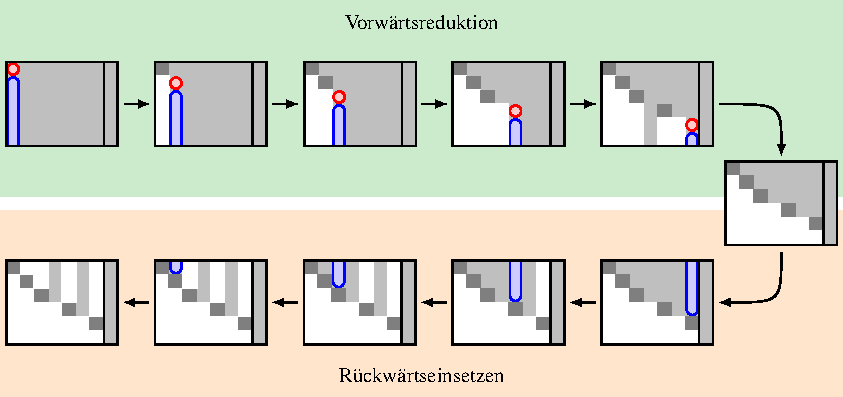
\includegraphics[width=\textwidth]{chapters/10-vektorenmatrizen/images/rref.pdf}
\caption{Zweckmässiger Ablauf der Berechnung des Gauss-Algorithmus.
Falls in einer Spalte kein weiteres von $0$ verschiedenes Pivotelement
zur Verfügung steht, wird die Zeile übersprungen.
Weisse Felder enthalten $0$, dunkelgraue $1$.
Die roten Kreise bezeichnen Pivot-Elemente, die blauen Felder
die mit einer Zeilensubtraktion zu $0$ gemacht werden sollen.
\label{buch:grundlagen:fig:gaussalgorithmus}}
\end{figure}
Die effizienteste Strategie für die Verwendung der beiden Operationen
ist in Abbildung~\ref{buch:grundlagen:fig:gaussalgorithmus} dargestellt.
In der Phase der {\em Vorwärtsreduktion} werden Pivotelemente von links
nach rechts möglichst auf der Diagonale gewählt und mit Zeilensubtraktionen
die darunterliegenden Spalten freigeräumt.
\index{Vorwärtsreduktion}%
Während des Rückwärtseinsetzens werden die gleichen Pivotelemente von 
rechts nach links genutzt, um mit Zeilensubtraktionen auch die
Spalten über den Pivotelemnten frei zu räumen.
\index{Rückwärtseinsetzen}%
Wenn in einer Spalte kein von $0$ verschiedenes Element als Pivotelement
zur Verfügung steht, wird diese Spalte übersprungen.
Die so erzeuge Tableau-Form heisst auch die {\em reduzierte Zeilenstufenform}
({\em reduced row echelon form}, RREF).
\index{reduzierte Zeilenstufenform}%
\index{reduced row echelon form}%

Da der Ablauf des Gauss-Algorithmus vollständig von den Koeffizienten der
Matrix $A$ bestimmt ist, kann er gleichzeitig für mehrere Spalten auf der
rechten Seite oder ganz ohne rechte Seite durchgeführt werden.

\subsubsection{Lösungsmenge}
\index{Lösungsmenge}%
Die Spalten, in denen im Laufe des Gauss-Algorithmus kein Pivotelement
gefunden werden kann, gehören zu Variablen, nach denen sich das
Gleichungssystem nicht auflösen lässt.
Diese Variablen sind daher nicht bestimmt, sie können beliebig gewählt
werden.
Alle anderen Variablen sind durch diese frei wählbaren Variablen
bestimmt.

Für ein Gleichungssystem $Ax=b$ mit Schlusstableau
\index{Schlusstableau}%
\begin{equation}
\begin{tabular}{|>{$}c<{$}>{$}c<{$}>{$}c<{$}>{$}c<{$}>{$}c<{$}>{$}c<{$}>{$}c<{$}>{$}c<{$}>{$}c<{$}>{$}c<{$}>{$}c<{$}|>{$}c<{$}|}
\hline
   x_1&   x_2&\dots &x_{j_i-1}&{\color{darkgreen}x_{j_1}}&x_{j_1+1}&\dots &x_{j_2-1}&{\color{darkgreen}x_{j_2}}&\dots&{\color{darkgreen}x_{j_k}}& \\
\hline
     1&     0&\dots &        0&c_{1j_1}   &     0&\dots &     0&c_{1j_2}     &\dots &c_{1j_k}     &d_1      \\
     0&     1&\dots &        0&c_{2j_1}   &     0&\dots &     0&c_{2j_2}     &\dots &c_{1j_k}     &d_2      \\[-2pt]
\vdots&\vdots&\ddots&\vdots   &\vdots     &\vdots&\ddots&\vdots&\vdots       &\ddots&\vdots       &\vdots   \\
     0&     0&\dots &        1&c_{i_1,j_1}&     0&\dots &     0&c_{i_1,j_2}  &\dots &c_{i_1j_k}   &d_{i_1}  \\
     0&     0&\dots &        0&          0&     1&\dots &     0&c_{i_1+1,j_2}&\dots &c_{i_1+1,j_k}&d_{i_1+1}\\[-2pt]
\vdots&\vdots&\ddots&\vdots   &\vdots     &\vdots&\vdots&\vdots&\vdots       &\ddots&\vdots       &\vdots   \\
     0&     0&\dots &        0&          0&     0&\dots &     1&c_{i_2,j_2}  &\dots &c_{i_2j_k}   &d_{i_2}  \\
     0&     0&\dots &        0&          0&     0&\dots &     0&            0&\dots &c_{i_2+1,j_k}&d_{i_2+1}\\[-2pt]
\vdots&\vdots&\ddots&\vdots   &\vdots     &\vdots&\ddots&\vdots&\vdots       &\ddots&\vdots       &\vdots   \\
     0&     0&\dots &        0&          0&     0&\dots &     0&            0&\dots &            0&d_{m}    \\
\hline
\end{tabular}
\end{equation}
mit den $k$ frei wählbaren Variablen
$x_{j_1}, x_{j_2},\dots, x_{j_k}$ kann die Lösungsmenge als
\[
\mathbb{L}
=
\left\{
\left.
\begin{pmatrix}
d_1\\
d_2\\
\vdots\\
d_{i_1}\\
d_{i_1+1}\\
\vdots\\
d_{i_2}\\
d_{i_2+1}\\
\vdots\\
d_{m}
\end{pmatrix}
+
{\color{darkgreen}x_{j_1}}
\begin{pmatrix}
-c_{1j_1}\\
-c_{2j_1}\\
\vdots\\
-c_{i_1,j_1}\\
{\color{darkgreen}1}\\
\vdots\\
0\\
0\\
\vdots\\
0\\
\end{pmatrix}
+
{\color{darkgreen}x_{j_1}}
\begin{pmatrix}
-c_{1j_2}\\
-c_{2j_2}\\
\vdots\\
-c_{j_1,j_2}\\
-c_{j_1+1,j_2}\\
\vdots\\
-c_{i_2,j_2}\\
{\color{darkgreen}1}\\
\vdots\\
0\\
\end{pmatrix}
+
\dots
+
{\color{darkgreen}x_{j_k}}
\begin{pmatrix}
-c_{1j_k}\\
-c_{2j_k}\\
\vdots\\
-c_{j_1,j_k}\\
-c_{j_1+1,j_k}\\
\vdots\\
-c_{i_2,j_k}\\
-c_{i_2+1,j_k}\\
\vdots\\
0\\
\end{pmatrix}
\;
\right|
{\color{darkgreen}x_{i_1}},{\color{darkgreen}x_{i_2}},\dots,{\color{darkgreen}x_{i_k}}\in\Bbbk
\right\}
\]
geschrieben werden.
Insbesondere ist die Lösungsmenge $k$-dimensional.

\subsubsection{Inverse Matrix}
Zu jeder quadratischen Matrix $A\in M_n(\Bbbk)$ kann man versuchen, die
Gleichungen
\[
Ac_1 = e_1,\quad Ac_2 = e_2, \dots, Ac_n = e_n
\]
mit den Standardbasisvektoren $e_i$ als rechten Seiten zu lösen, wobei
die $c_i$ Vektoren in $\Bbbk^n$ sind.
Diese Vektoren kann man mit Hilfe des Gauss-Algorithmus finden:
\[
\begin{tabular}{|>{$}c<{$}>{$}c<{$}>{$}c<{$}>{$}c<{$}|>{$}c<{$}>{$}c<{$}>{$}c<{$}>{$}c<{$}|}
\hline
a_{11}&a_{12}&\dots &a_{1n}&1     &0     &\dots &0     \\
a_{21}&a_{22}&\dots &a_{2n}&0     &1     &\dots &0     \\
\vdots&\vdots&\ddots&\vdots&\vdots&\vdots&\ddots&\vdots\\
a_{n1}&a_{n2}&\dots &a_{nn}&0     &0     &\dots &1     \\
\hline
\end{tabular}
\rightarrow
\begin{tabular}{|>{$}c<{$}>{$}c<{$}>{$}c<{$}>{$}c<{$}|>{$}c<{$}>{$}c<{$}>{$}c<{$}>{$}c<{$}|}
\hline
1     &0     &\dots &0     &c_{11}&c_{12}&\dots &c_{1n}\\
0     &1     &\dots &0     &c_{21}&c_{22}&\dots &c_{2n}\\
\vdots&\vdots&\ddots&\vdots&\vdots&\vdots&\ddots&\vdots\\
0     &0     &\dots &1     &c_{n1}&c_{n2}&\dots &c_{nn}\\
\hline
\end{tabular}
\]
Die Vektoren $c_k$ sind die Spaltenvektoren der Matrix $C$ mit den
Einträgen $c_{ij}$.

Mit den Vektoren $c_k$ können jetzt beliebige inhomogene Gleichungssysteme
$Ax=b$ gelöst werden.
Da $b = b_1e_1 + b_2e_2 + \dots + b_ne_n$, kann man die Lösung $x$ als
$x = b_1c_1+b_2c_2+\dots+b_nc_n$ konstruieren.
Tatsächlich gilt
\begin{align*}
Ax
&= 
A( b_1c_1+b_2c_2+\dots+b_nc_n)
\\
&=
b_1Ac_1 + b_2Cc_2 + \dots + b_nAc_n
\\
&=
b_1e_1 + b_2e_2 + \dots + b_ne_n
=
b.
\end{align*}
Die Linearkombination $x=b_1c_1+\dots+b_nc_n$ kann in Vektorform als $x=Cb$
geschrieben werden.

Die Konstruktion von $C$ bedeutet auch, dass $AC=E$, daher heisst $C$ auch
die zu $A$ {\em inverse Matrix}.
\index{inverse Matrix}
Sie wird auch $C=A^{-1}$ geschrieben.

Die Definition der inversen Matrix stellt sicher, dass $AA^{-1}=I$ gilt,
daraus folgt aber noch nicht, dass auch $A^{-1}A=I$ ist.
Diese Eigenschaft kann man jedoch wie folgt erhalten.
Sei $C$ die inverse Matrix von $A$, also $AC=I$.
Sei weiter $D$ die inverse Matrix von $C$, also $CD=I$.
Dann ist zunächst $A=AE=A(CD)=(AC)D=ID=D$ und weiter
$CA=CD=I$.
Mit der Bezeichnung $C=A^{-1}$ erhalten wir also auch $A^{-1}A=I$.

Die Eigenschaften der Matrizenmultiplikation stellen sicher,
dass die Menge der invertierbaren Matrizen eine Struktur bilden,
die man Gruppe nennt, die in Abschnitt~\ref{buch:grundlagen:subsection:gruppen}
genauer untersucht wird.
In diesem Zusammenhang wird dann auf
Seite~\pageref{buch:vektorenmatrizen:satz:gruppenregeln}
die Eigenschaft $A^{-1}A=I$ ganz allgemein gezeigt.

\subsubsection{Determinante}
XXX TODO

%
% Lineare Abbildungen
%
\subsection{Lineare Abbildungen
\label{buch:grundlagen:subsection:lineare-abbildungen}}
Der besondere Nutzen der Matrizen ist, dass sie auch lineare Abbildungen
zwischen Vektorräumen beschreiben können.
In diesem Abschnitt werden lineare Abbildungen abstrakt definiert
und die Darstellung als Matrix mit Hilfe einer Basis eingeführt.


\subsubsection{Definition}
Eine lineare Abbildung zwischen Vektorräumen muss so gestaltet sein,
dass die Operationen des Vektorraums erhalten bleiben.
Dies wird von der folgenden Definition erreicht.

\begin{definition}
Eine Abbildung $f\colon V\to U$ zwischen Vektorräumen $V$ und $U$
heisst linear, wenn
\[
\begin{aligned}
f(v+w) &= f(v) + f(w)&&\forall v,w\in V 
\\
f(\lambda v) &= \lambda f(v) &&\forall v\in V,\lambda \in \Bbbk
\end{aligned}
\]
gilt.
\end{definition}

Lineare Abbildungen sind in der Mathematik sehr verbreitet.

\begin{beispiel}
Sie $V=C^1([a,b])$ die Menge der stetig differenzierbaren Funktionen 
auf dem Intervall $[a,b]$ und $U=C([a,b])$ die Menge der
stetigen Funktion aif $[a,b]$. 
Die Ableitung $\frac{d}{dx}$ macht aus einer Funktion $f(x)$ die
Ableitung $f'(x)$.
Die Rechenregeln für die Ableitung stellen sicher, dass 
\[
\frac{d}{dx}
\colon
C^1([a,b]) \to  C([a,b]) 
:
f \mapsto f'
\]
eine lineare Abbildung ist.
\end{beispiel}

\begin{beispiel}
Sei $V$ die Menge der Riemann-integrierbaren Funktionen auf dem
Intervall $[a,b]$ und $U=\mathbb{R}$.
Das bestimmte Integral
\[
\int_a^b \;\colon V \to U : f \mapsto \int_a^b f(x)\,dx
\]
ist nach den bekannten Rechenregeln für bestimmte Integrale
eine lineare Abbildung.
\end{beispiel}

\subsubsection{Matrix}
Um mit linearen Abbildungen rechnen zu können, ist eine Darstellung 
mit Hilfe von Matrizen nötig.
Sei also $\mathcal{B}=\{b_1,\dots,b_n\}$ eine Basis von $V$ und
$\mathcal{C} = \{ c_1,\dots,c_m\}$ eine Basis von $U$.
Das Bild des Basisvektors $b_i$ kann als Linearkombination der
Vektoren $c_1,\dots,c_m$ dargestellt werden.
Wir verwenden die Bezeichnung
\[
f(b_i) 
=
a_{1i} c_1 + \dots + a_{mi} c_m.
\]
Die lineare Abbildung $f$ bildet den Vektor $x$ mit Koordinaten
$x_1,\dots,x_n$ ab auf 
\begin{align*}
f(x)
&=
f(x_1b_1  + \dots x_nb_n)
\\
&=
x_1 f(b_1) + \dots x_nf(b_n)
\\
&=
x_1(a_{11} c_1 + \dots + a_{m1} c_m)
+
\dots
+
x_n(a_{1n} c_1 + \dots + a_{mn} c_m)
\\
&=
( a_{11} x_1 + \dots + a_{1n} x_n ) c_1
+
\dots
+
( a_{m1} x_1 + \dots + a_{mn} x_n ) c_m
\end{align*}
Die Koordinaten von $f(x)$ in der Basis $\mathcal{C}$ in $U$ sind 
also gegeben durch das Matrizenprodukt $Ax$, wenn $x$ der Spaltenvektor
aus den Koordinaten in der Basis $\mathcal{B}$ in $V$ ist.

Die Matrix einer linearen Abbildung macht Aussagen über eine lineare
Abbilung der Rechnung zugänglich.
Allerdings hängt die Matrix einer linearen Abbildung von der Wahl der
Basis ab.
Gleichzeitig ist dies eine Chance, durch Wahl einer geeigneten Basis
kann man eine Matrix in eine Form bringen, die zur Lösung eines
Problems optimal geeignet ist.

\subsubsection{Basiswechsel}
In einem Vektorraum $V$ seien zwei Basen $\mathcal{B}=\{b_1,\dots,b_n\}$
und $\mathcal{B}'=\{b_1',\dots,b_n'\}$ gegeben.
Ein Vektor $v\in V$ kann in beiden beiden Basen dargestellt werden.
Wir bezeichnen mit dem Spaltenvektor $x$ die Koordinaten von $v$ in der
Basis $\mathcal{B}$ und mit dem Spaltenvektor $x'$ die Koordinaten
in der Basisi $\mathcal{B}'$.
Um die Koordinaten umzurechnen, muss man die Gleichung
\begin{equation}
x_1b_1 + \dots + x_nb_n = x_1'b_1' + \dots + x_n'b_n'
\label{buch:vektoren-und-matrizen:eqn:basiswechselgleichung}
\end{equation}
lösen.

Stellt man sich die Vektoren $b_i$ und $b_j'$ als $m$-dimensionale
Spaltenvektoren vor mit $m\ge n$, dann bekommt
\eqref{buch:vektoren-und-matrizen:eqn:basiswechselgleichung}
die Form eines Gleichungssystems
\[
\begin{linsys}{6}
b_{11}x_1&+& \dots &+&b_{1n}x_n&=&b_{11}'x_1'&+& \dots &+&b_{1n}'x_n'\\
\vdots   & & \ddots& &\vdots   & &\vdots     & & \ddots& &\vdots     \\
b_{m1}x_1&+& \dots &+&b_{mn}x_n&=&b_{m1}'x_1'&+& \dots &+&b_{mn}'x_n'
\end{linsys}
\]
Dieses Gleichungssystem kann man mit Hilfe eines Gauss-Tableaus lösen.
Wir schreiben die zugehörigen Variablen 
\[
\renewcommand{\arraystretch}{1.1}
\begin{tabular}{|>{$}c<{$} >{$}c<{$} >{$}c<{$}|>{$}c<{$}>{$}c<{$}>{$}c<{$}|}
\hline
x_1&\dots&x_n&x_1'&\dots&x_n'\\
\hline
b_{11}&\dots &b_{1n}&b_{11}'&\dots &v_{1n}'\\
\vdots&\ddots&\vdots&\vdots &\ddots&\vdots \\
b_{n1}&\dots &b_{nn}&b_{n1}'&\dots &v_{nn}'\\
\hline
b_{n+1,1}&\dots &b_{n+1,n}&b_{n+1,1}'&\dots &v_{n+1,n}'\\
\vdots&\ddots&\vdots&\vdots &\ddots&\vdots \\
b_{m1}&\dots &b_{mn}&b_{m1}'&\dots &v_{mn}'\\
\hline
\end{tabular}
\rightarrow
\begin{tabular}{|>{$}c<{$} >{$}c<{$} >{$}c<{$}|>{$}c<{$}>{$}c<{$}>{$}c<{$}|}
\hline
x_1&\dots&x_n&x_1'&\dots&x_n'\\
\hline
1     &\dots &0     &t_{11}             &\dots              &t_{1n}        \\
\vdots&\ddots&\vdots&\vdots             &\ddots             &\vdots        \\
0     &\dots &1     &t_{n1}             &\dots              &t_{nn}        \\
\hline
0     &\dots &0     &{\color{red}0}     &{\color{red}\dots} &{\color{red}0}\\
\vdots&\ddots&\vdots&{\color{red}\vdots}&{\color{red}\ddots}&{\color{red}\vdots}\\
0     &\dots &0     &{\color{red}0}     &{\color{red}\dots} &{\color{red}0}\\
\hline
\end{tabular}
\]
Das rechte untere Teiltableau enthält lauter Nullen genau dann, wenn jeder
Vektor in $V$ sich in beiden Mengen $\mathcal{B}$ und $\mathcal{B}'$
ausdrücken lässt.
Dies folgt aber aus der Tatsache, dass $\mathcal{B}$ und $\mathcal{B}'$
beide Basen sind, also insbesondere den gleichen Raum aufspannen.
Die $n\times n$-Matrix $T$ mit Komponenten $t_{ij}$ rechnet Koordinaten
in der Basis $\mathcal{B}'$ um in Koordinaten in der Basis $\mathcal{B}$.

\subsubsection{Umkehrabbbildung}
Sei $f$ eine umkehrbare lineare Abbildung $U\to V$ und $g\colon V\to U$.
die zugehörige Umkehrabbildung.
Für zwei Vektoren $u$ und $w$ in $U$ gibt es daher Vektoren $a=g(u)$
und $b=g(w)$ in $V$ derart, dass $f(a)=u$ und $f(b)=w$.
Weil $f$ linear ist, folgt daraus $f(a+b)=u+w$ und $f(\lambda a)=\lambda a$
für jedes $\lambda\in\Bbbk$.
Damit kann man jetzt 
\begin{align*}
g(u+w)&=g(f(a)+f(b)) = g(f(a+b)) = a+b = g(u)+g(w)
\\
g(\lambda u) &= g(\lambda f(a))=g(f(\lambda a)) = \lambda a = \lambda g(u)
\end{align*}
berechnen, was zeigt, dass auch $g$ eine lineare Abbildung ist.
Hat $f$ in geeignet gewählten Basen die Matrix $F$, dann hat die
Umkehrabbildung $g=f^{-1}$ die Matrix $G=F^{-1}$.
Da auch $f(g(y))=y$ gilt für jeden Vektor $y\in V$ folgt, dass $FF^{-1}=E$
und $F^{-1}F=E$.

\subsubsection{Kern und Bild}
Für die Eindeutigkeit der Lösung eines linearen Gleichungssytems
ist entscheidend, ob das zugehörige homogene Gleichungssystem $Ax=0$
eine nichttriviale Lösung hat.
Seine Lösungmenge spielt also eine besondere Rolle, was rechtfertigt,
ihr einen Namen zu geben.

\begin{definition}
\index{Kern}%
Ist $f$ eine lineare Abbildung $U\to V$, dann heisst die Menge
\[
\ker f
=
\{x\in U\;|\; f(x)=0\}
\]
der {\em Kern} oder {\em Nullraum} der linearen Abbildung $f$.
Ist $A \in M_{m\times n}(\Bbbk)$ Matrix, dann gehört dazu eine lineare
Abbildung $f\colon\Bbbk^n\to\Bbbk^m$.
Der Kern oder Nullraum der Matrix $A$ ist die Menge
\[
\ker A
=
\{ x\in\Bbbk^m \;|\; Ax=0\}.
\]
\end{definition}

Der Kern ist ein Unterraum, denn für zwei Vektoren $u,w\in \ker f$ 
\[
\begin{aligned}
f(u+v)&=f(u) + f(v) = 0+0 = 0 &&\Rightarrow& u+v&\in\ker f\\
f(\lambda u)&=\lambda f(u) = \lambda\cdot 0=0&&\Rightarrow& \lambda u&\in\ker f
\end{aligned}
\]
gilt.

Ob ein Gleichungssystem $Ax=b$ überhaupt eine Lösung hat, hängt davon,
ob der Vektor $b$ als Bild der durch $A$ beschriebenen linearen Abbildung
$\Bbbk^n \to \Bbbk^m$ enthalten ist.
Wir definieren daher das Bild einer linearen Abbildung oder Matrix.

\begin{definition}
Ist $f\colon V\to U$ eine lineare Abbildung dann ist das Bild von $f$
der Unterraum 
\[
\operatorname{im}f = \{ f(v)\;|\;v\in V\} \subset U
\]
von $U$.
Das Bild einer $m\times n$-Matrix $A$ ist die Menge
\[
\operatorname{im}A = \{ Av \;|\; v\in\Bbbk^n\} \subset \Bbbk^m.
\]
\end{definition}

Zwei Vektoren $a,b\in\operatorname{im} f$ haben Urbilder $u,w\in V$ mit
$f(u)=a$ und $f(w)=b$.
Für Summe und Multiplikation mit Skalaren folgt
\[
\begin{aligned}
a+b&= f(u)+f(v)=f(u+v) &&\Rightarrow a+b\in\operatorname{im}f\\
\lambda a&=\lambda f(u) = f(\lambda u) &&\Rightarrow \lambda a&\in\operatorname{im}f,
\end{aligned}
\]
also ist auch das Bild $\operatorname{im}f$ ein Unterraum von $U$.
Das Bild der Matrix $A$ ist der Unterraum
\[
\{ x_1f(b_1) + \dots x_n f(b_n) | x_i\in\Bbbk\}
=
\langle f(b_1),\dots,f(b_n)\rangle
=
\langle a_1,\dots,a_n\rangle
\]
von $\Bbbk^m$, aufgespannt von den Spaltenvektoren $a_i$ von $A$.

\subsubsection{Rang und Defekt}
Die Dimensionen von Bild und Kern sind wichtige Kennzahlen einer Matrix.
\begin{definition}
Sei $A$ eine Matrix $A\in M_{m\times n}(\Bbbk)$.
Der {\em Rang} der Matrix $A$ ist die Dimension des Bildraumes von $A$:
$\operatorname{rank}A=\dim\operatorname{im} A$.
\index{Rang einer Matrix}%
Der {\em Defekt} der Matrix $A$ ist die Dimension des Kernes von $A$:
$\operatorname{def}A=\dim\ker A$.
\index{Defekt einer Matrix}%
\end{definition}

Da der Kern mit Hilfe des Gauss-Algorithmus bestimmt werden kann,
können Rang und Defekt aus dem Schlusstableau 
eines homogenen Gleichungssystems mit $A$ als Koeffizientenmatrix
abgelesen werden.

\begin{satz}
Ist $A\in M_{m\times n}(\Bbbk)$ eine $m\times n$-Matrix,
dann gilt
\[
\operatorname{rank}A
=
n-\operatorname{def}A.
\]
\end{satz}

\subsubsection{Quotient}
TODO: $\operatorname{im} A \simeq \Bbbk^m/\ker A$
